\level{2}{Applicazione Android}
	\begin{figure}[H]\centering
        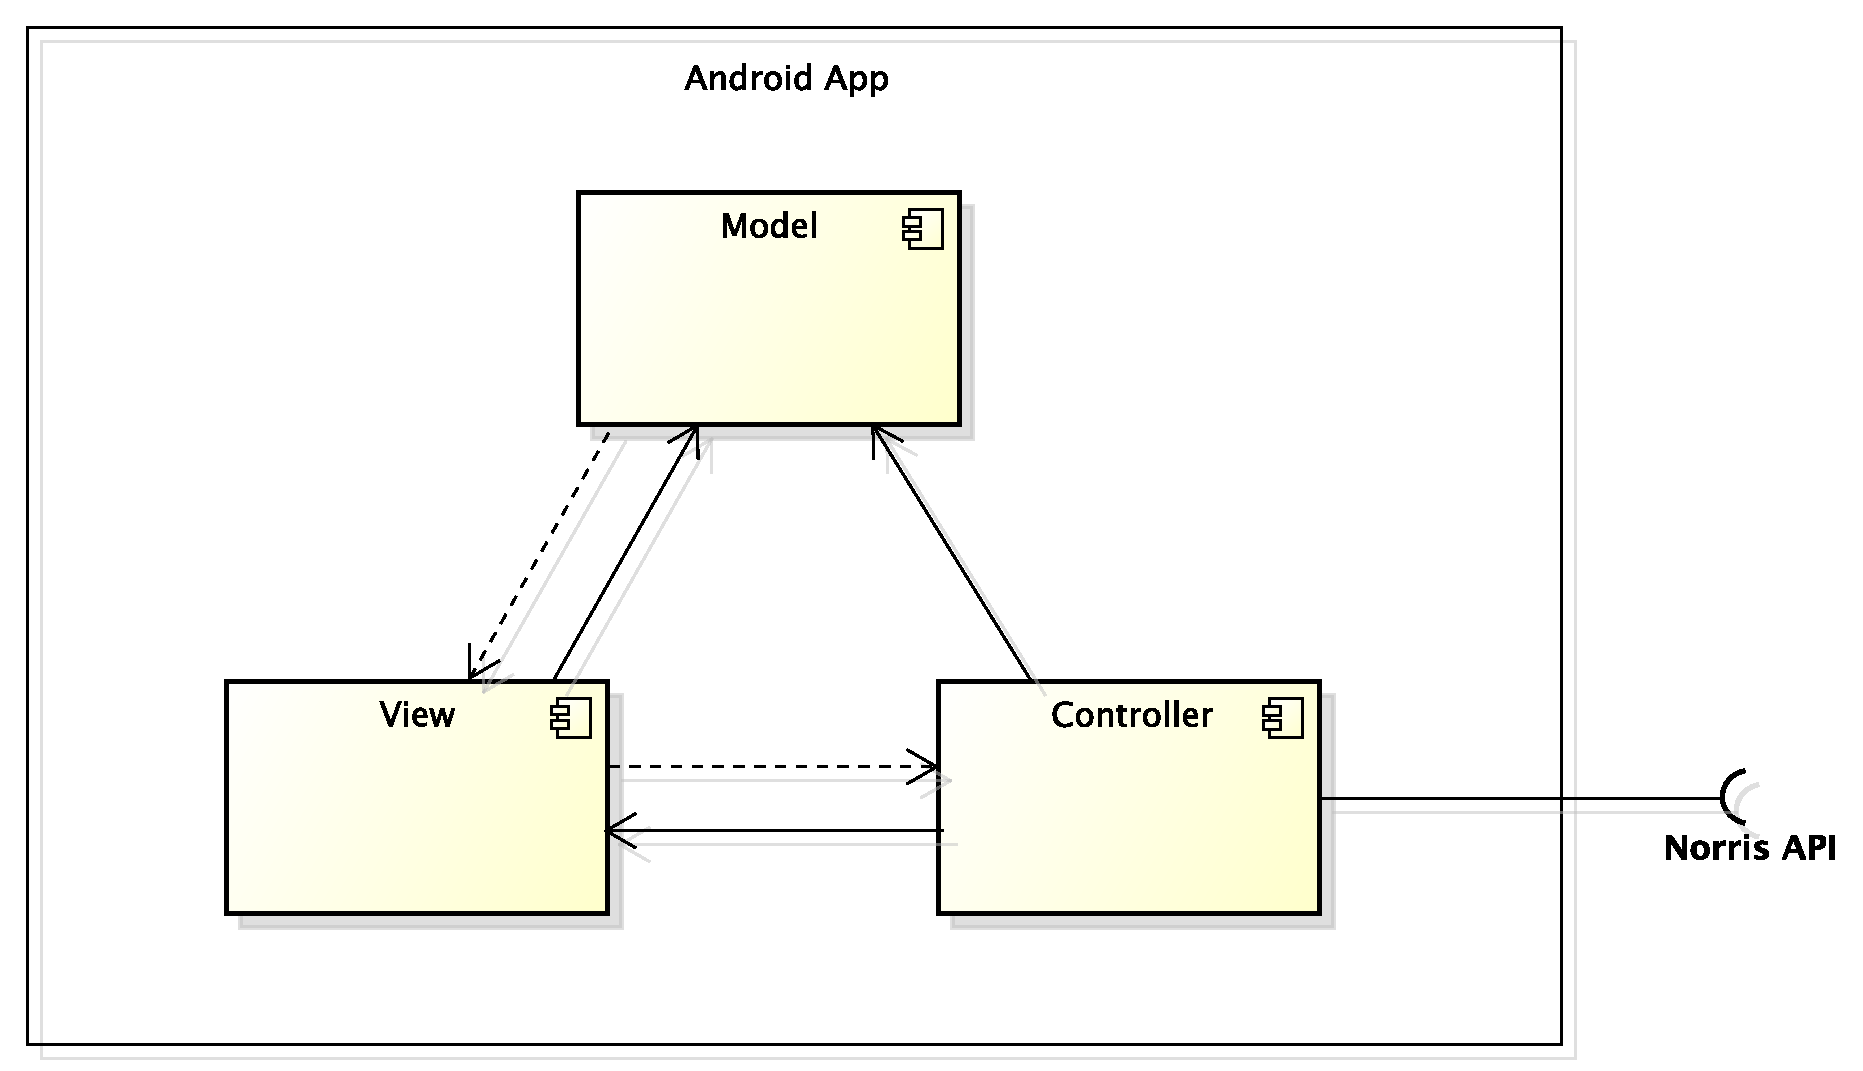
\includegraphics[width=\textwidth]{SpecificaTecnica/Pics/ComponentiApplicazione}
        \caption{Diagramma delle componenti dell'Applicazione Android}
    \end{figure}
	\level{3}{Design Pattern utilizzati}
	Nella progettazione delle componenti dell'applicazione Android abbiamo deciso di utilizzare il design pattern MVC, in quanto favorisce il disaccoppiamento delle classi e di conseguenza la robustezza, la modularità e la manutenibilità del codice. \\
Il pattern MVC, inoltre, risulta particolarmente adatto per la realizzazione del prodotto in quanto è previsto l'impiego di più viste per un unico modello di dati, che è lo scopo principale dell'MVC.
    \level{3}{Descrizione delle componenti principali della app}
    	\level{4}{Model} 
        Il Model è la componente che rappresenta l'astrazione dei grafici visualizzati nell'applicazione. In essa sono contenuti i dati riguardanti i grafici, assieme alle relative impostazioni. In particolare sono presenti i modelli di tutte le tipologie di chart implementati da Norris. Il Data Model fornisce per ciascuna tipologia di grafico i metodi per inserire i dati e configurare alcune impostazioni. 
    
       \level{4}{View}
        La View è il componente che rappresenta le varie UI dell'applicazione e i vari widget dei grafici da inserire nelle UI. In tale componente potrebbero esser sollevati degli eventi scatenati dall'utente.
       \level{4}{Controller}
        Questo componente ha il compito di gestire tutto il controllo dell'applicazione. Le operazioni che esso gestisce sono riassunte nel seguente elenco:
        	\begin{itemize}
        		\item creazione del modello qualora questo sia necessario;
        		\item utilizzo delle API esterne di Norris;
        		\item interpretazione dei pacchetti ricevuti dal server contenenti i dati delle richieste API;
        		\item ascolto sul canale socket per ricevere gli aggiornamenti di stato dei chart;
        		\item interpretazione dei pacchetti di aggiornamento;
        		\item richiesta al modello di aggiornare il proprio stato;
        		\item richiesta della creazione dei widget dei grafici da inserire nelle UI dell'applicazione;
        		\item avvio delle varie activity dell'applicazione;
        		\item gestione delle gesture dell'utente.
        \end{itemize}
    \level{3}{Descrizione delle interazioni che i componenti dell'app hanno tra di loro}
    	Le interazioni tra i componenti sono rappresentati con una freccia. Sono presenti due tipologie di frecce:
    	\begin{itemize}
    			\item{continua: } rappresenta l'invocazione di un metodo;
    			\item{tratteggiata: } rappresenta lo scatenarsi di un evento.
    		\end{itemize}

    	Riportiamo di seguito la descrizione di ogni interazione.

    	\level{4}{View - Controller}
        In seguito all'esecuzione di una gesture da parte dell'utente, la View notifica il Controller tramite l'emissione dell'evento opportuno. Il Controller si occupa quindi di gestire quest'ultimo. Questa interazione si verifica in particolare quando l'utente seleziona un item della lista dei grafici presenti nell'istanza di Norris richiesta.

	    \level{4}{Controller - Model}
	    Il Controller richiede al Model di modificare il proprio stato. Ciò avviene per esempio subito dopo l'utilizzo dell'API esterna di Norris per richiedere un grafico o in seguito all'arrivo di un pacchetto di aggiornamento.

	    \level{4}{Model - View}
	    Il Model notifica le View che lo osservano ogniqualvolta il suo stato viene modificato. Tale interazione è neccessaria per mantenere coerenza tra il modello e la sua rappresentazione nella View. 

	    \level{4}{View - Model}
	   	Questa interazione rappresenta la richiesta dello stato del Model da parte della View. Viene effettuata quando la View ha la necessità di esporre i dati del Model o qualcosa che sia dipendente dallo stato di quest'ultimo. Ciò si verifica per esempio subito dopo che la View ha ricevuto la notifica di aggiornamento da parte del modello.

	    \level{4}{Controller - View}
	   	Tale interazione rappresenta la richiesta da parte del Controller di visualizzare una specifica Activity. Ciò avviene ad ogni necessità di cambiare Activity.

